\chapter{Конструкторский раздел}
\section{Диаграмма проектируемой базы данных}
На рисунке~\ref{fig:BD} представлена диаграмма  проектируемой базы данных.

\begin{figure}
	\centering
	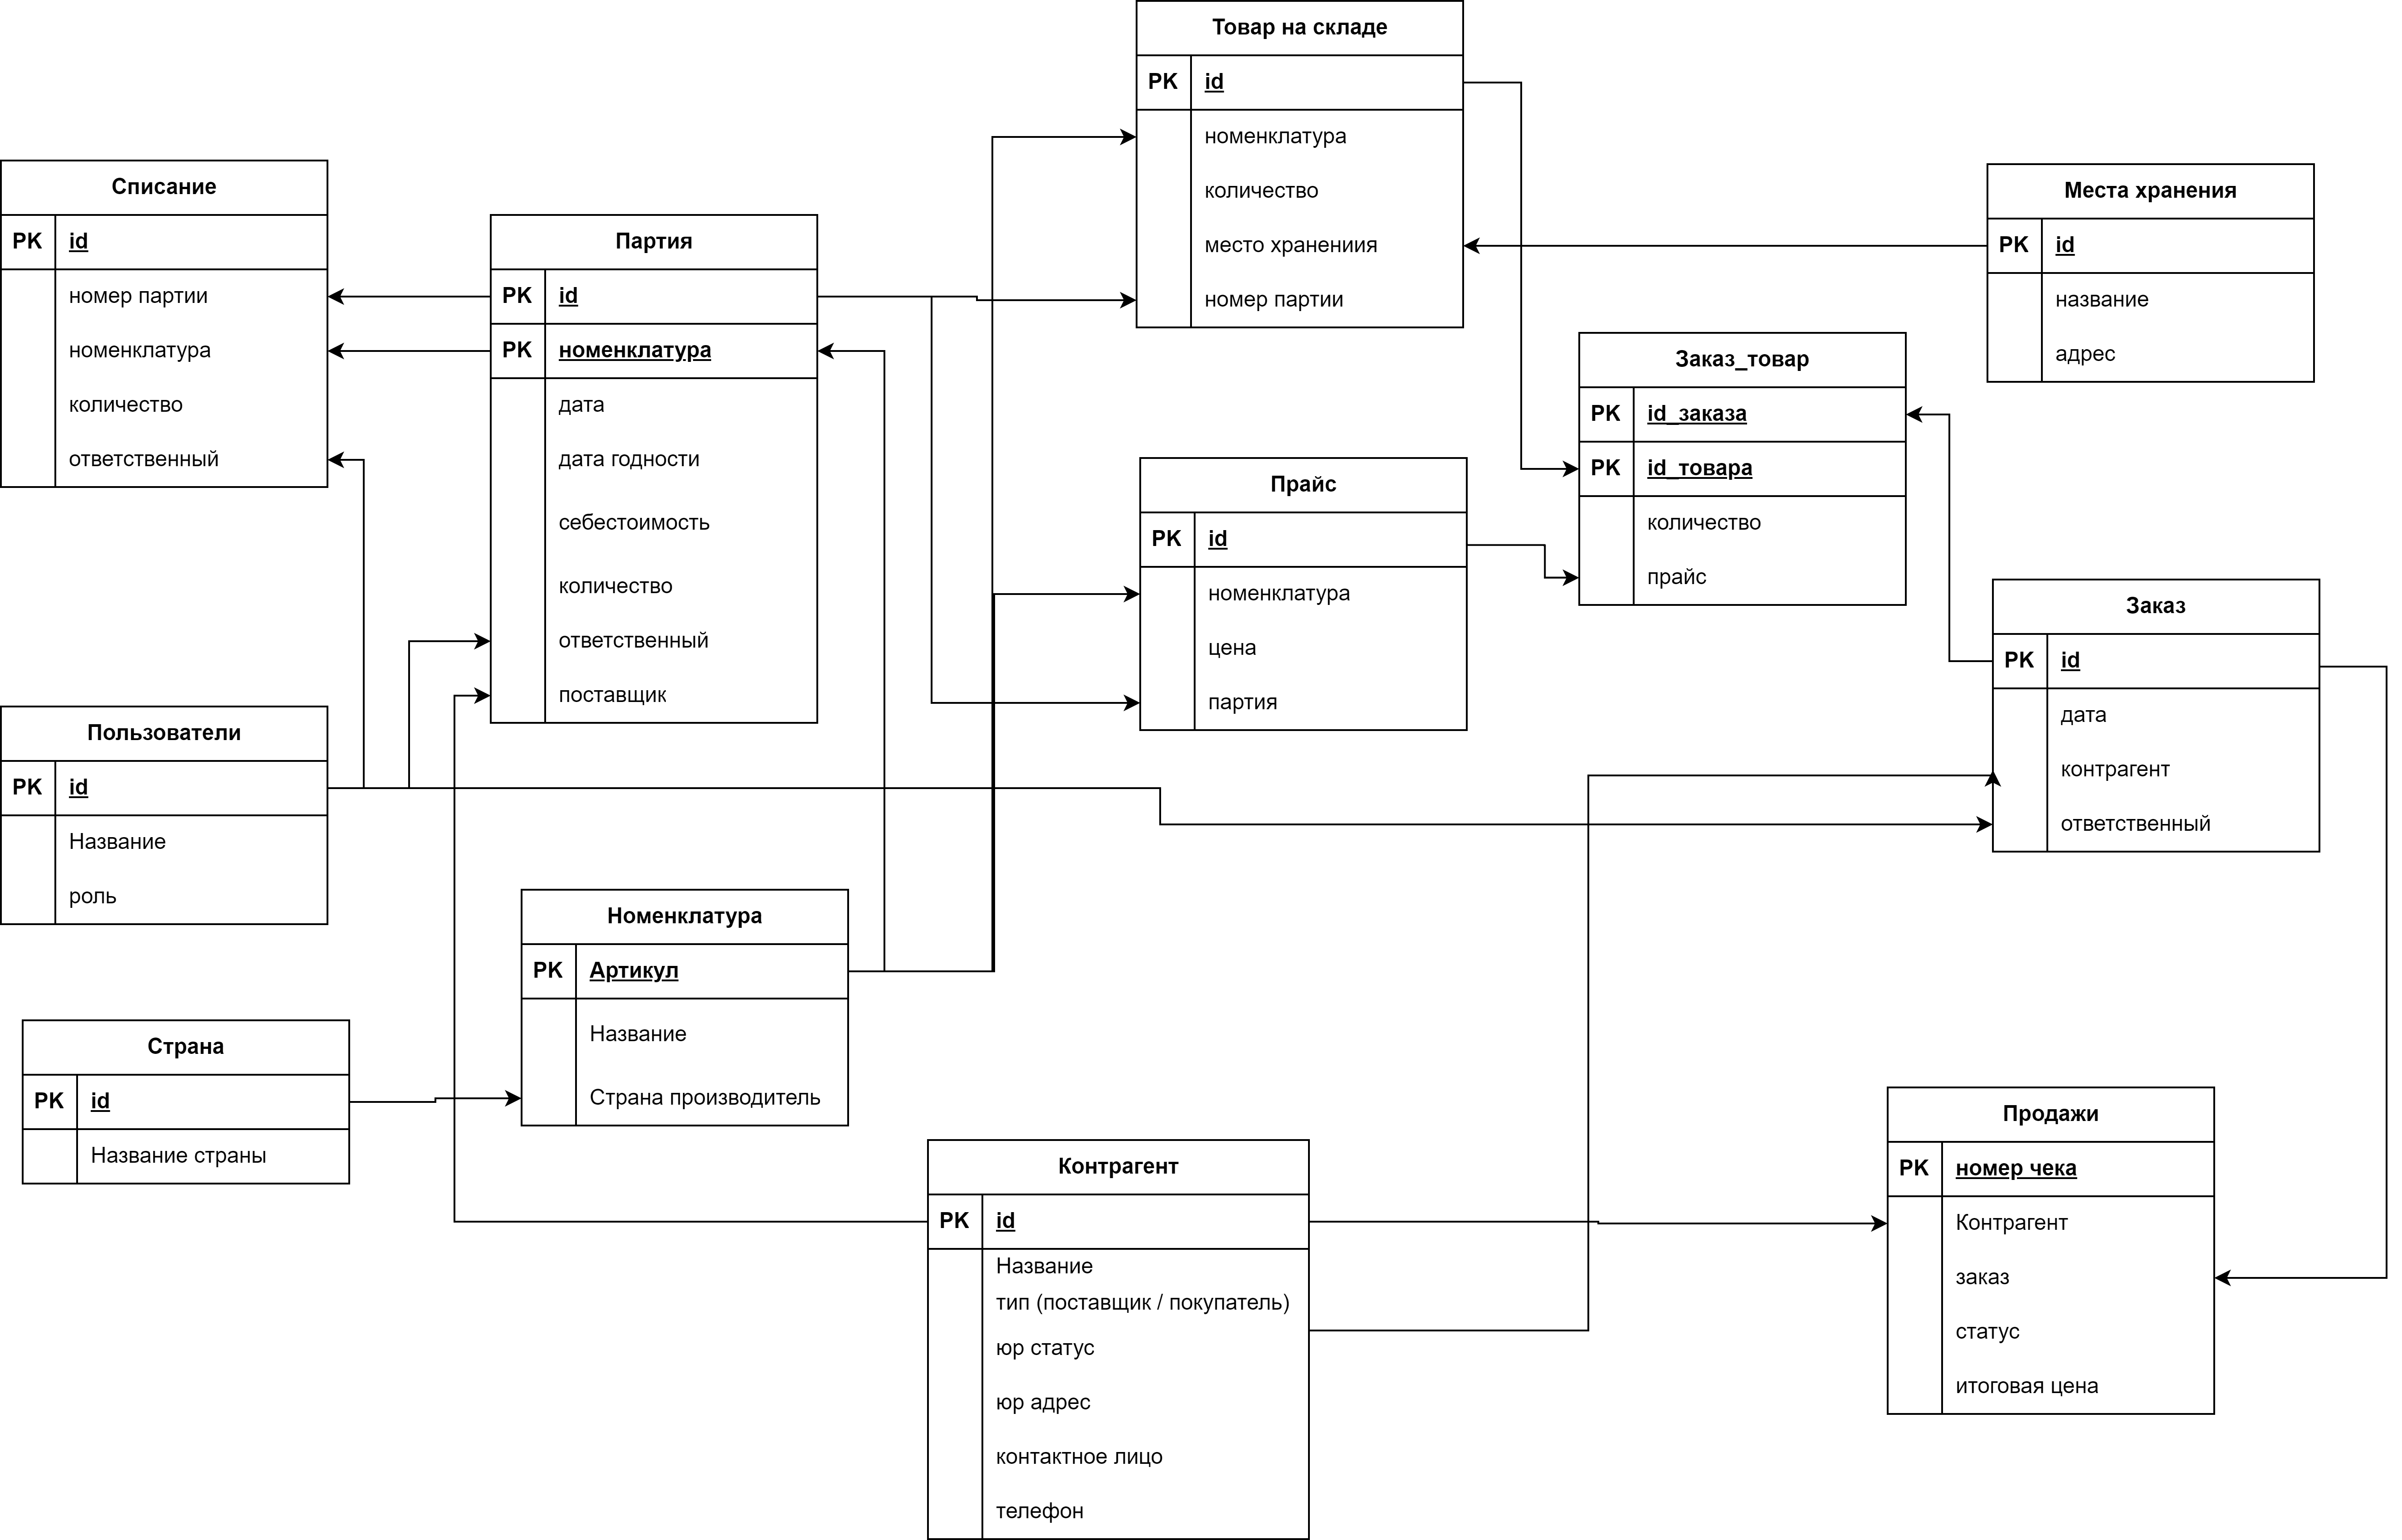
\includegraphics[width=1.5\linewidth, angle=-90]{pictures/BD_2}
	\caption{Диаграмма проектируемой базы данных}
	\label{fig:BD}
\end{figure}

\section{Описание сущностей проектируемой базы данных}
\begin{itemize}
	\item \textbf{Списание}
	\begin{itemize}
		\item Основная сущность для учёта списания товаров
		\item Атрибуты:
		\begin{itemize}
			\item id - уникальный идентификатор
			\item номер партии
			\item номенклатура
			\item количество списываемого товара
			\item ответственный за списание (пользователь с ролью кладовщик)
		\end{itemize}
	\end{itemize}
	
	\item \textbf{Пользователь}
	\begin{itemize}
		\item Сущность для хранения данных пользователей системы
		\item Атрибуты:
		\begin{itemize}
			\item id - уникальный идентификатор
			\item название (имя пользователя)
			\item роль в системе
		\end{itemize}
	\end{itemize}
	
	\item \textbf{Страна}
	\begin{itemize}
		\item Справочник стран
		\item Атрибуты:
		\begin{itemize}
			\item id - уникальный идентификатор
			\item название страны
		\end{itemize}
	\end{itemize}
	
	\item \textbf{Товар на складе}
	\begin{itemize}
		\item Сущность учёта текущих остатков на складе
		\item Атрибуты:
		\begin{itemize}
			\item id - уникальный идентификатор
			\item номенклатура
			\item количество товара
			\item место хранения
			\item номер партии
		\end{itemize}
	\end{itemize}
	
	\item \textbf{Заказ}
	\begin{itemize}
		\item Сущность для оформления заказов
		\item Атрибуты:
		\begin{itemize}
			\item id - уникальный идентификатор
			\item дата
			\item контрагент
			\item ответственный за заказ
		\end{itemize}
	\end{itemize}
	
	\item \textbf{Заказ товар}
	\begin{itemize}
		\item Сущность для сопоставления заказа и товаров
		\item Атрибуты:
		\begin{itemize}
			\item id заказа
			\item id товара
			\item количество
			\item прайс
		\end{itemize}
	\end{itemize}
	
	\item \textbf{Контрагент}
	\begin{itemize}
		\item Сущность для хранения данных контрагентов
		\item Атрибуты:
		\begin{itemize}
			\item id - уникальный идентификатор
			\item название
			\item тип (поставщик/покупатель)
			\item юридический статус
			\item юридический адрес
			\item контактное лицо
			\item телефон
		\end{itemize}
	\end{itemize}
	
	\item \textbf{Продажи}
	\begin{itemize}
		\item Сущность для учёта продаж
		\item Атрибуты:
		\begin{itemize}
			\item номер чека
			\item контрагент
			\item заказ
			\item статус продажи
			\item итоговая цена
		\end{itemize}
	\end{itemize}
	
	\item \textbf{Место хранения}
	\begin{itemize}
		\item Справочник складских помещений
		\item Атрибуты:
		\begin{itemize}
			\item id - уникальный идентификатор
			\item название места хранения
			\item адрес
		\end{itemize}
	\end{itemize}
	
	\item \textbf{Номенклатура}
	\begin{itemize}
		\item Основной справочник товаров/продукции
		\item Атрибуты:
		\begin{itemize}
			\item id - уникальный идентификатор
			\item название товара
			\item страна производства
		\end{itemize}
	\end{itemize}
	
	\item \textbf{Партия}
	\begin{itemize}
		\item Учёт поступлений товаров партиями
		\item Атрибуты:
		\begin{itemize}
			\item id - уникальный идентификатор
			\item дата
			\item дата годности
			\item себестоимость
			\item количество
			\item ответственный
			\item поставщик
		\end{itemize}
	\end{itemize}
	
	\item \textbf{Прайс}
	\begin{itemize}
		\item Справочник цен на товары
		\item Атрибуты:
		\begin{itemize}
			\item id - уникальный идентификатор
			\item номенклатура
			\item цена
			\item партия
		\end{itemize}
	\end{itemize}
\end{itemize}

\section{Описание проектируемых ограничений целостности базы данных}
В таблице~\ref{tab:constraints} приведены ограничения целостности проектируемой базы данных.
\begin{table}[h]
	\centering
	\caption{Ограничения в таблицах базы данных}
	\label{tab:constraints}
	\begin{tabular}{|l|p{11cm}|}
		\hline
		\textbf{Таблица} & \textbf{Описание} \\
		\hline
		Страна & Длина названия страны должна быть больше 0 \\
		\hline
		Номенклатура & Длина названия номенклатуры должна быть больше 0 \\
		\cline{2-2}
		& Поле country\_id не может быть NULL \\
		\hline
		Контрагент & Длина названия контрагента должна быть больше 0 \\
		\cline{2-2}
		& Длина имени контактного лица должна быть больше 0 \\
		\cline{2-2}
		& Телефон должен соответствовать формату (+ необязателен, затем от 10 до 15 цифр) \\
		\hline
		Пользователь & Длина имени пользователя должна быть больше 1 \\
		\hline
		Партия товаров & Дата производства не может быть будущей \\
		\cline{2-2}
		& Срок годности должен быть после даты производства \\
		\cline{2-2}
		& Себестоимость должна быть положительной \\
		\cline{2-2}
		& Количество должно быть положительным \\
		\hline
		Списание & Количество списания не может быть отрицательным \\
		\hline
		Цена & Цена продажи должна быть положительной \\
		\hline
		Место хранения & Длина названия места хранения должна быть больше 0 \\
		\hline
		Товар на складе & Количество на складе не может быть отрицательным \\
		\hline
		Связь заказа и товара & Внешний ключ на таблицу product\_in\_stock \\
		\cline{2-2}
		& Внешний ключ на таблицу order \\
		\hline
		Продажи & Итоговая цена должна быть положительной \\
		\hline
	\end{tabular}
\end{table}

\section{Описание всех проектируемых процедур/функций/триггеров в формате схемы}
На рисунках~\ref{fig:trigger1} и \ref{fig:trigger2} представлены диаграммы алгоритмов триггера на обновление товара на складе при поступлении новой партии товара и триггера на обновление товара на складе при покупке, соответственно.
\begin{figure}
	\centering
	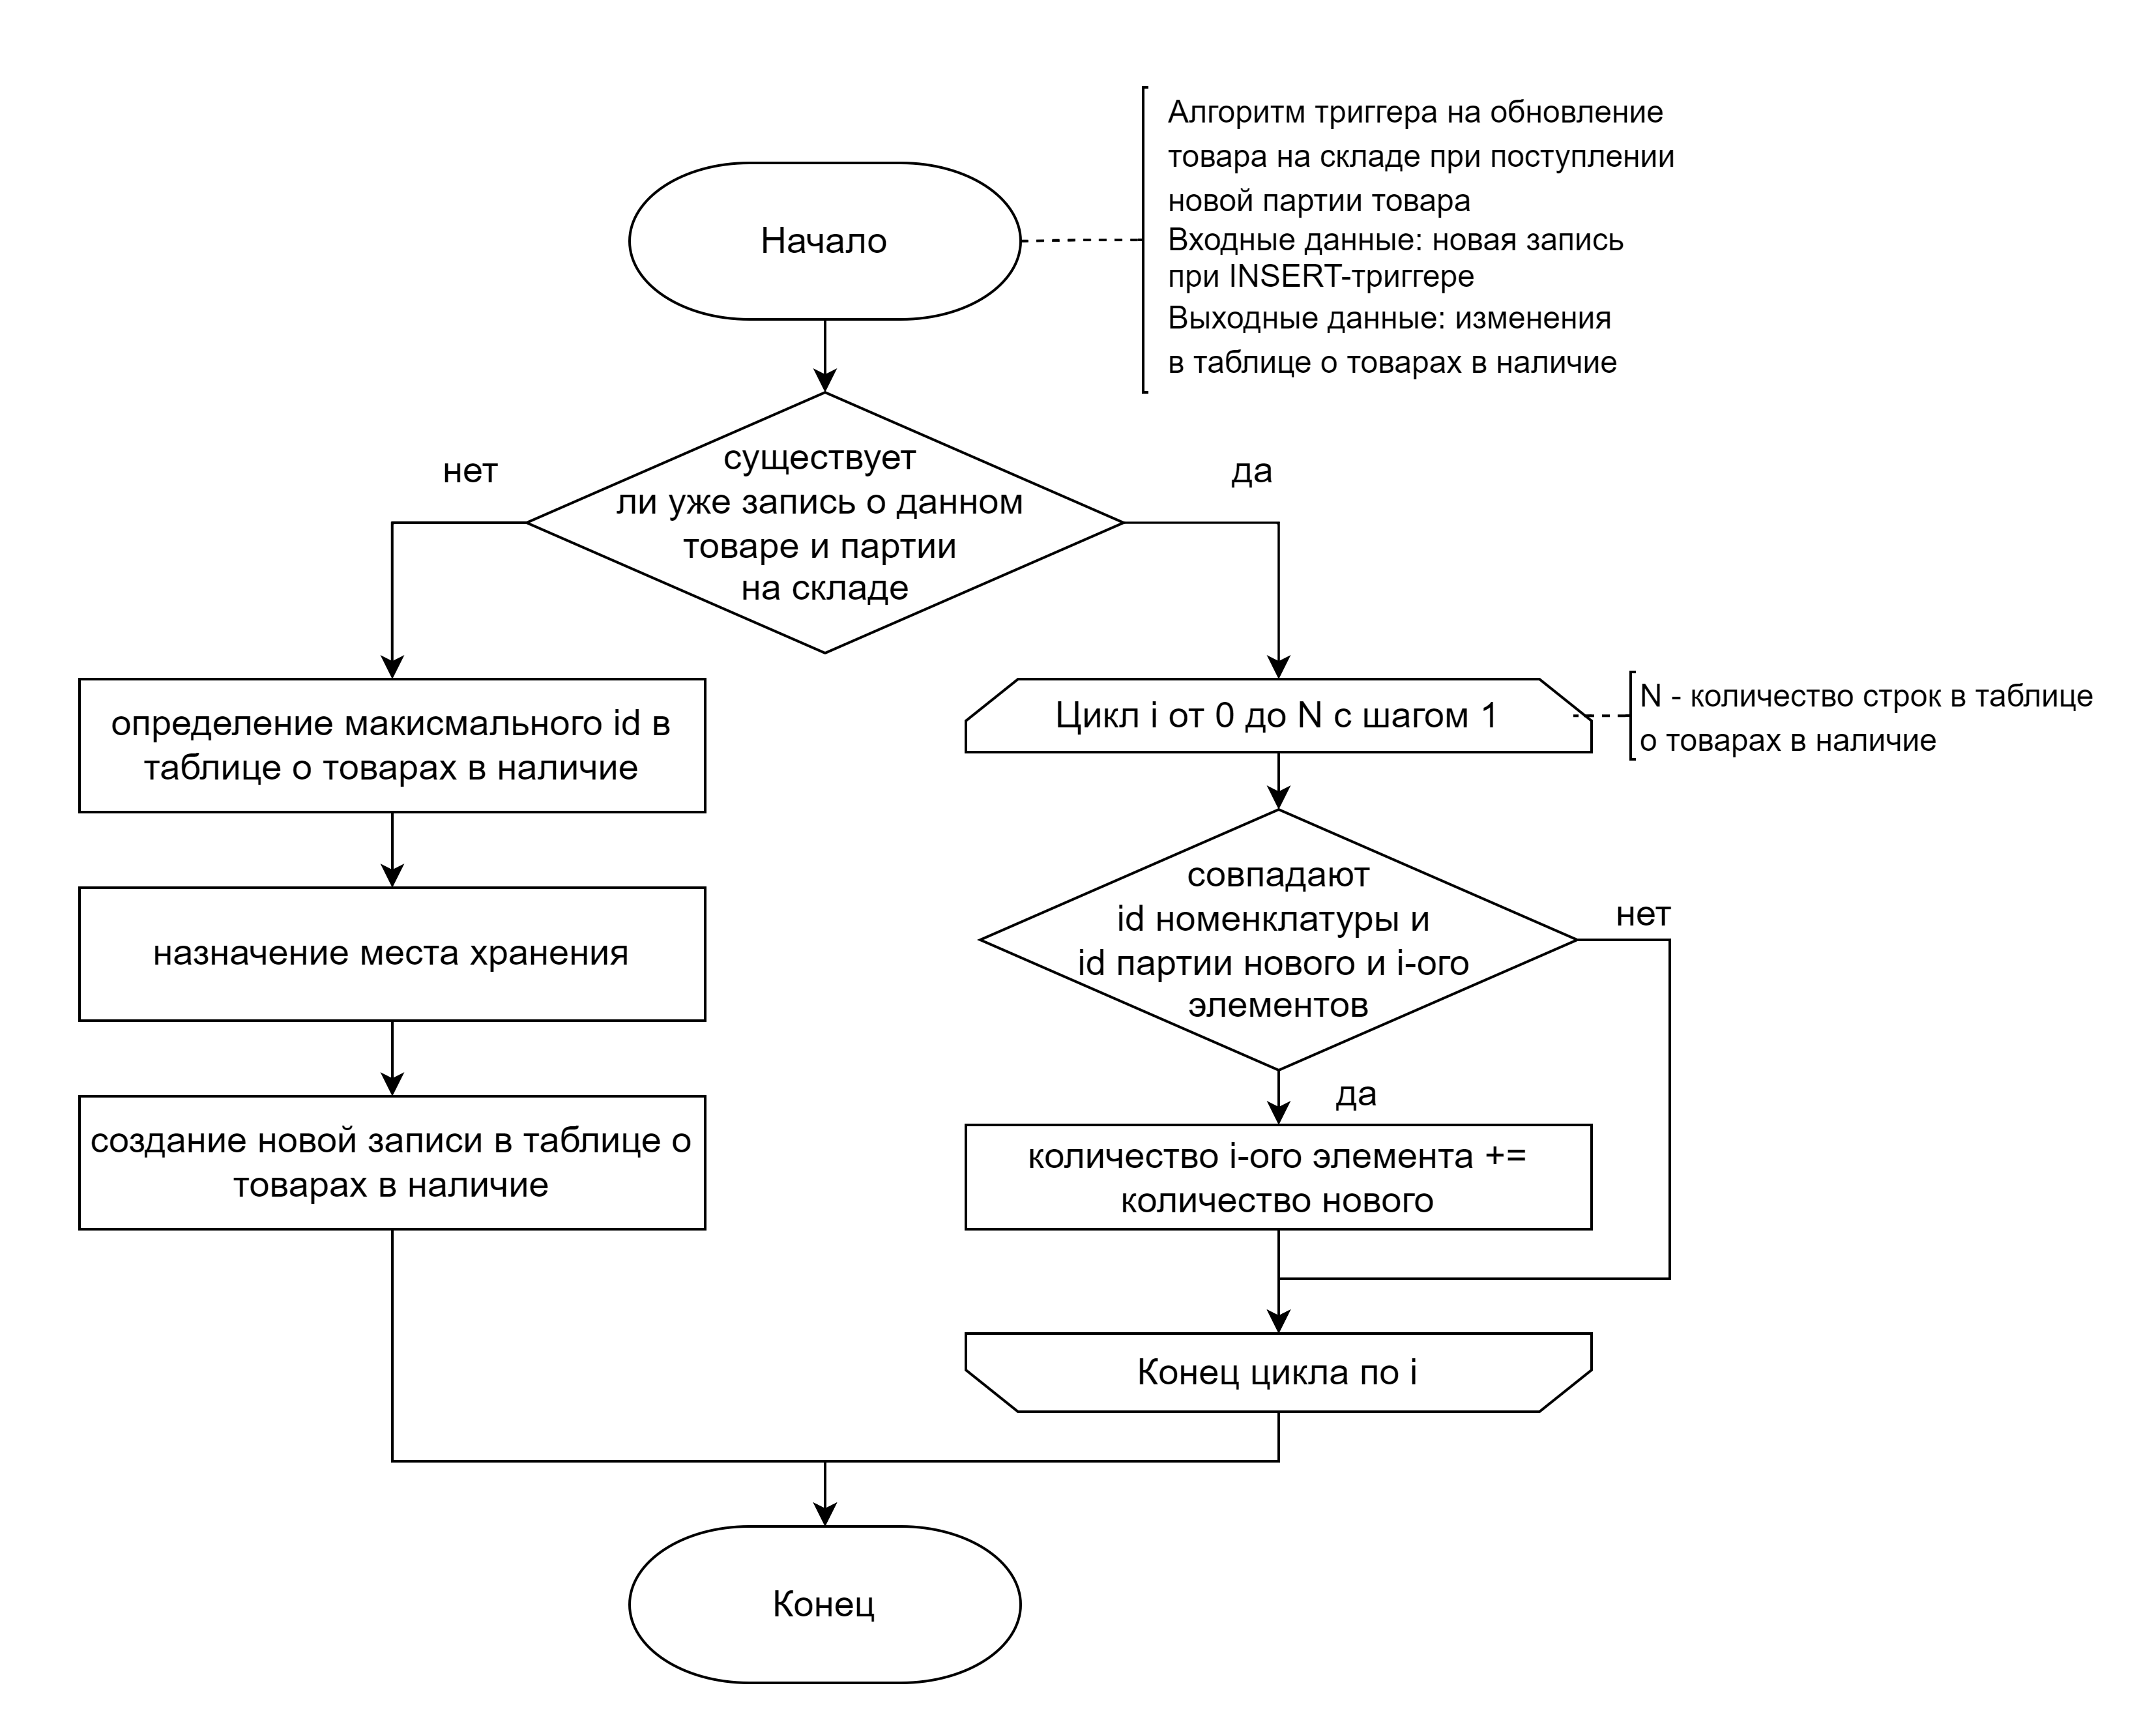
\includegraphics[width=1\linewidth]{pictures/trigger_1_load_batch}
	\caption{Диаграмма алгоритма триггера на обновление товара на складе при поступлении новой партии товара}
	\label{fig:trigger1}
\end{figure}
\begin{figure}
	\centering
	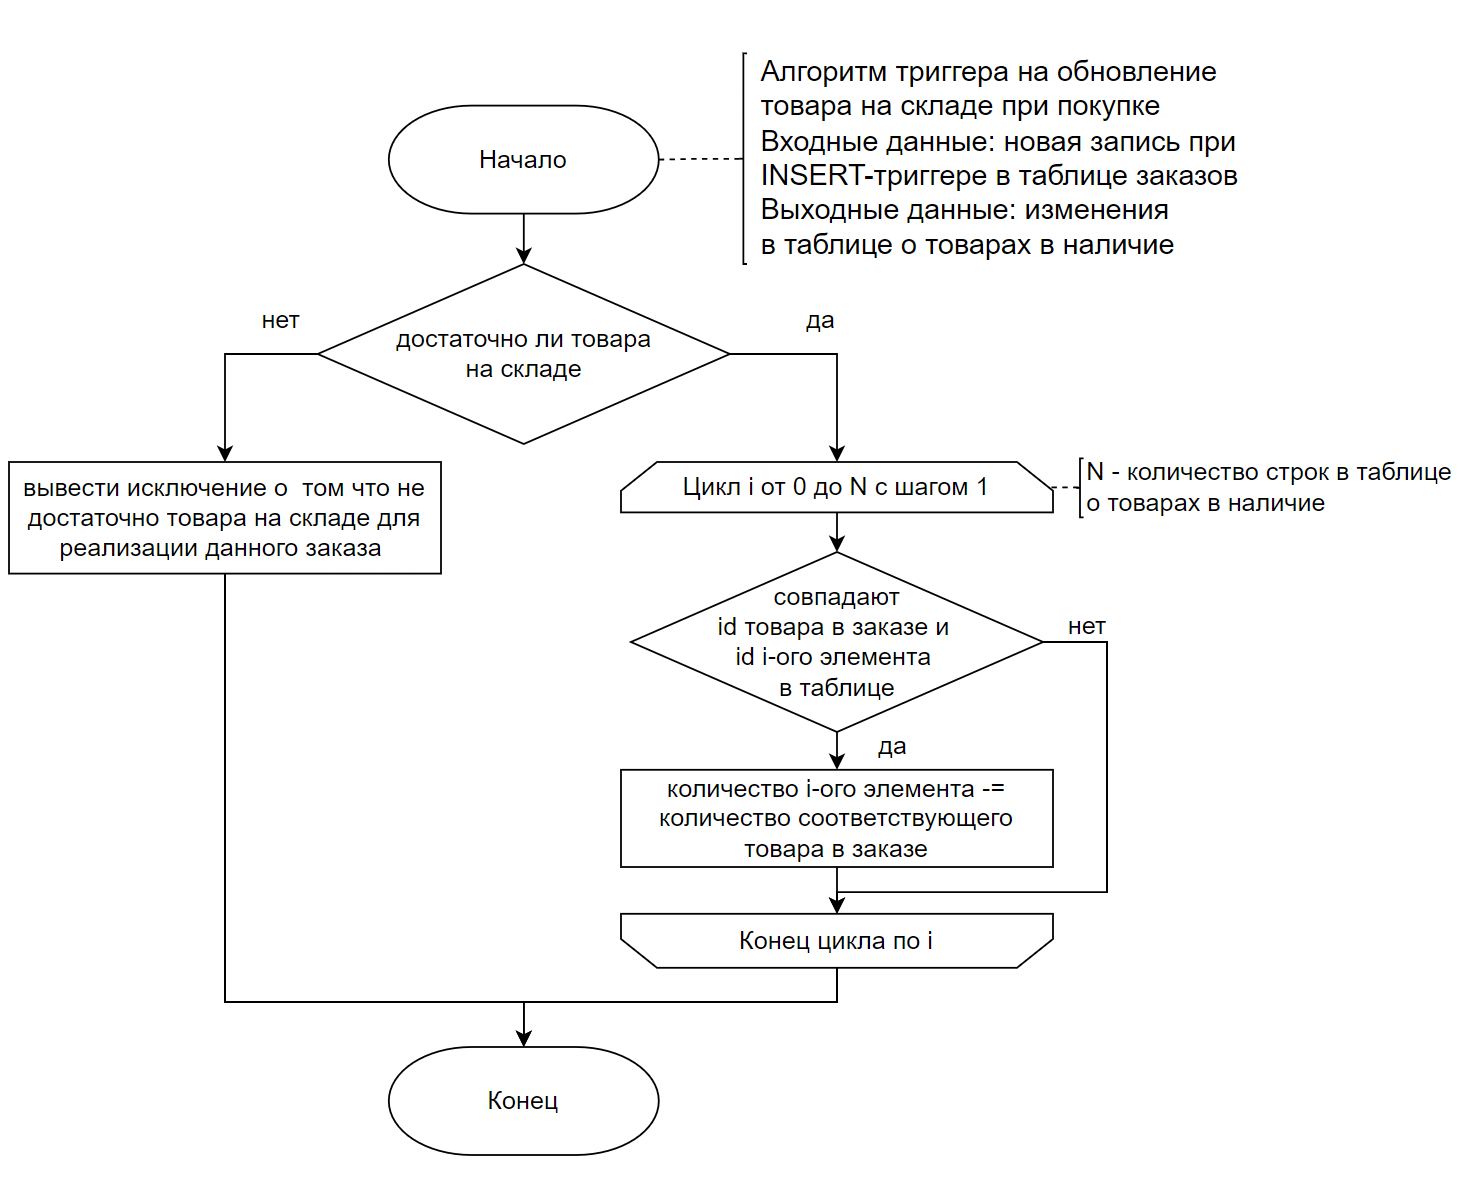
\includegraphics[width=1\linewidth]{pictures/trigger_2_make_purchase}
	\caption{Диаграмма алгоритма триггера на обновление товара на складе при покупке}
	\label{fig:trigger2}
\end{figure}
\section{Описание проектируемой ролевой модели на уровне базы данных}
Три имеющиеся типа пользователей обладают следующим набором прав. Кладовщики -- загрузка информации  о партии и просмотр каталога доступных товаров; продавцы -- внесение информации о заказах и продажах, просмотр каталога доступных товаров; администраторы -- всё выше перечисленное. 
\section*{Вывод}
\addcontentsline{toc}{section}{Вывод}
В конструкторском разделе была разработана структура базы данных, включающая 12 нормализованных сущностей, связанных между собой через внешние ключи, что обеспечивает целостность данных. Диаграмма базы данных наглядно демонстрирует взаимосвязи между таблицами: от справочников (номенклатура, страны, места хранения) до операционных сущностей (партии, заказы, продажи, списания). Особое внимание уделено механизмам поддержания актуальности данных через систему триггеров, автоматически обновляющих остатки на складе при поступлении новых партий и продажах. Ролевая модель, реализованная на уровне СУБД, разделяет права доступа между тремя типами пользователей (администраторами, продавцами и кладовщиками), обеспечивая безопасность и соответствие бизнес-процессам компании.